\documentclass[a4paper, czech]{article}

\usepackage[czech]{babel}
\usepackage{indentfirst}
\usepackage{graphicx}
\usepackage{float}
\usepackage[margin=1.5cm]{geometry}
\usepackage{booktabs}
\usepackage{amsmath}
\usepackage[dvipsnames]{xcolor}
\usepackage{multirow}
\usepackage{tabularray}
\usepackage{bold-extra}
\usepackage{circuitikz}
\usepackage{caption}
\usepackage{subcaption}
\usepackage[utf8]{inputenc}
\usepackage{array}

\begin{document}
\begin{table}[H]
    \centering
    \begin{tblr}{
        cell{1}{1} = {c = 2, r = 4}{c}, % Logo
        cell{1}{4} = {c = 3}{c}, % Předmět
        cell{2}{4} = {c = 3}{c}, % Jméno
        cell{3}{4} = {}{c}, % Ročník
        cell{3}{6} = {}{c}, % Studijní skupina
        cell{4}{4} = {}{c}, % Spolupracoval
        cell{4}{6} = {}{c}, % Mereno dne
        cell{5}{1} = {c = 2}{55mm}, % Kontroloval
        cell{5}{3} = {c = 2}{55mm}, % Hodnoceni
        cell{5}{5} = {c = 2}{55mm}, % Dne
        cell{6}{2} = {c = 5}{}, % Nazev ulohy
        cell{7}{1} = {}{c}, % Číslo úlohy
        cell{7}{2} = {c = 5}{c}, % Název úlohy
        vline{1,2,7} = {1.2pt},
        vline{3,5},
        hline{1,5,6,8} = {1.2pt},
        hline{2,3,4}
        }
        
\includegraphics{logo_fekt.png} & & \textsuperscript{Předmět} & \large \textbf{Měření v audiotechnice} \\
             & & \textsuperscript{Jméno} & \large \textbf{Karolína Šebestová} \\
             & & \textsuperscript{Ročník} & \large \textbf{3.} & \textsuperscript{Studijní skupina} & \large \textbf{St 14:00} \\
             & & \textsuperscript{Spolupracoval} & \large \textbf{Filip Kokavec} & \textsuperscript{Měřeno dne} & \large \textbf{27.11.2024} \\
        \textsuperscript{Kontroloval} & & \textsuperscript{Hodnocení} & & \textsuperscript{Dne} \\
        \textsuperscript{Číslo úlohy} & \textsuperscript{Název úlohy} \\
        \Large \textbf{9A} & \Large \textsc{\textbf{Měření parametrů technické cívky wattmetrem}} \\
    \end{tblr}
\end{table}

\section{Zadání}

\begin{itemize}
    \item Změřte závislost impedance výkonové tlumivky na sycení.
\end{itemize}

\section{Teoretický úvod}

\section{Výsledky měření}

\subsection{Tabulky}

\begin{table}[H]
    \catcode`\-=12
    \centering
    \caption{Měření technické cívky wattmetrem}
    \renewcommand{\arraystretch}{1.25}
    \begin{tabular}{ccccccccccccc}
        \toprule
        $I$   & \multicolumn{3}{c}{$I_1$} & \multicolumn{3}{c}{$I_2$} & \multicolumn{3}{c}{$U$} & \multicolumn{3}{c}{$P'$}           \\
        \cmidrule(rl){1-1}
        \cmidrule(rl){2-4}
        \cmidrule(rl){5-7}
        \cmidrule(rl){8-10}
        \cmidrule(rl){11-13}
        A   & $\alpha_\text{A1}$  & $k_\text{A1}$      & A    & $\alpha_\text{A1}$  & $k_\text{A1}$    & A    & $\alpha_\text{V}$  & $k_\text{V}$      & V    & $\alpha_\text{W}$  & $k_\text{W}$                  & W     \\
        \midrule
        0,9 & 0,9  & $\frac{1,2}{1,2}$  & 0,9  & 5      & 6/6    & 5    & 41   & 60/60   & 41   & 72 & $5 \frac{75}{75} \cdot 0,2 \frac{1}{5}$ & 14,40 \\
        0,8 & 0,8  & $\frac{1,2}{1,2}$  & 0,8  & 4      & 6/6    & 4    & 40   & 60/60   & 40   & 56 & $5 \frac{75}{75} \cdot 0,2 \frac{1}{5}$ & 11,20 \\
        0,6 & 0,6  & $\frac{1,2}{1,2}$  & 0,6  & 3      & 6/6    & 3    & 37   & 60/60   & 37   & 32 & $5 \frac{75}{75} \cdot 0,2 \frac{1}{5}$ & 6,400 \\
        0,4 & 0,4  & $\frac{0,6}{0,6}$  & 0,4  & 2      & 6/6    & 2    & 34   & 60/60   & 34   & 38 & $5 \frac{30}{75} \cdot 0,2 \frac{1}{5}$ & 3,040 \\
        0,2 & 0,2  & $\frac{0,6}{0,6}$  & 0,2  & 1      & 6/6    & 1    & 30   & 60/60   & 30   & 28 & $5 \frac{15}{75} \cdot 0,2 \frac{1}{5}$ & 1,120 \\
        \bottomrule
    \end{tabular}
\end{table}
\begin{table}[H]
    \catcode`\-=12
    \centering
    \begin{tabular}{ccccccccccc}
        \toprule
        $I$   & $R_\text{WU}$   & $R_\text{V}$   & $\Delta_P$    & $P$     & $\Delta_I$    & $I$     & $R_\text{S}$    & $L_\text{S}$    & $R_\text{P}$    & $L_\text{P}$    \\
        \cmidrule(rl){1-1}
        \cmidrule(rl){2-2}
        \cmidrule(rl){3-3}
        \cmidrule(rl){4-4}
        \cmidrule(rl){5-5}
        \cmidrule(rl){6-6}
        \cmidrule(rl){7-7}
        \cmidrule(rl){8-8}
        \cmidrule(rl){9-9}
        \cmidrule(rl){10-10}
        \cmidrule(rl){11-11}
        A   & $\Omega$     & $\Omega$    & W     & W     & A     & A     & $\Omega$     & H     & $\Omega$     & H     \\
        \midrule
        0,9 & 15000 & 6000 & 0,392 & 14,01 & 0,010 & 0,890 & 17,67 & 0,135 & 120,0 & 0,159 \\
        0,8 & 15000 & 6000 & 0,373 & 10,83 & 0,009 & 0,791 & 17,32 & 0,151 & 147,8 & 0,171 \\
        0,6 & 15000 & 6000 & 0,319 & 6,081 & 0,009 & 0,591 & 17,39 & 0,191 & 225,1 & 0,207 \\
        0,4 & 6000  & 6000 & 0,385 & 2,655 & 0,011 & 0,389 & 17,57 & 0,273 & 435,5 & 0,284 \\
        0,2 & 3000  & 6000 & 0,450 & 0,670 & 0,015 & 0,185 & 19,58 & 0,512 & 1 343 & 0,520 \\
        \bottomrule
        \multicolumn{11}{c}{$\delta_\text{TPW} = 1\,\%$; $\delta_\text{TP\,MTP} = 0,2\,\%$; $\delta_\text{TPV} = 0,5\,\%$; $\delta_\text{TPA} = 0,5\,\%$; $R_\text{WU} = 200\,\Omega/\text{V}$; $R_\text{V} = 6000\,\Omega$}
    \end{tabular}
\end{table}

\subsection{Grafy}

\begin{figure}[H]
    \centering
    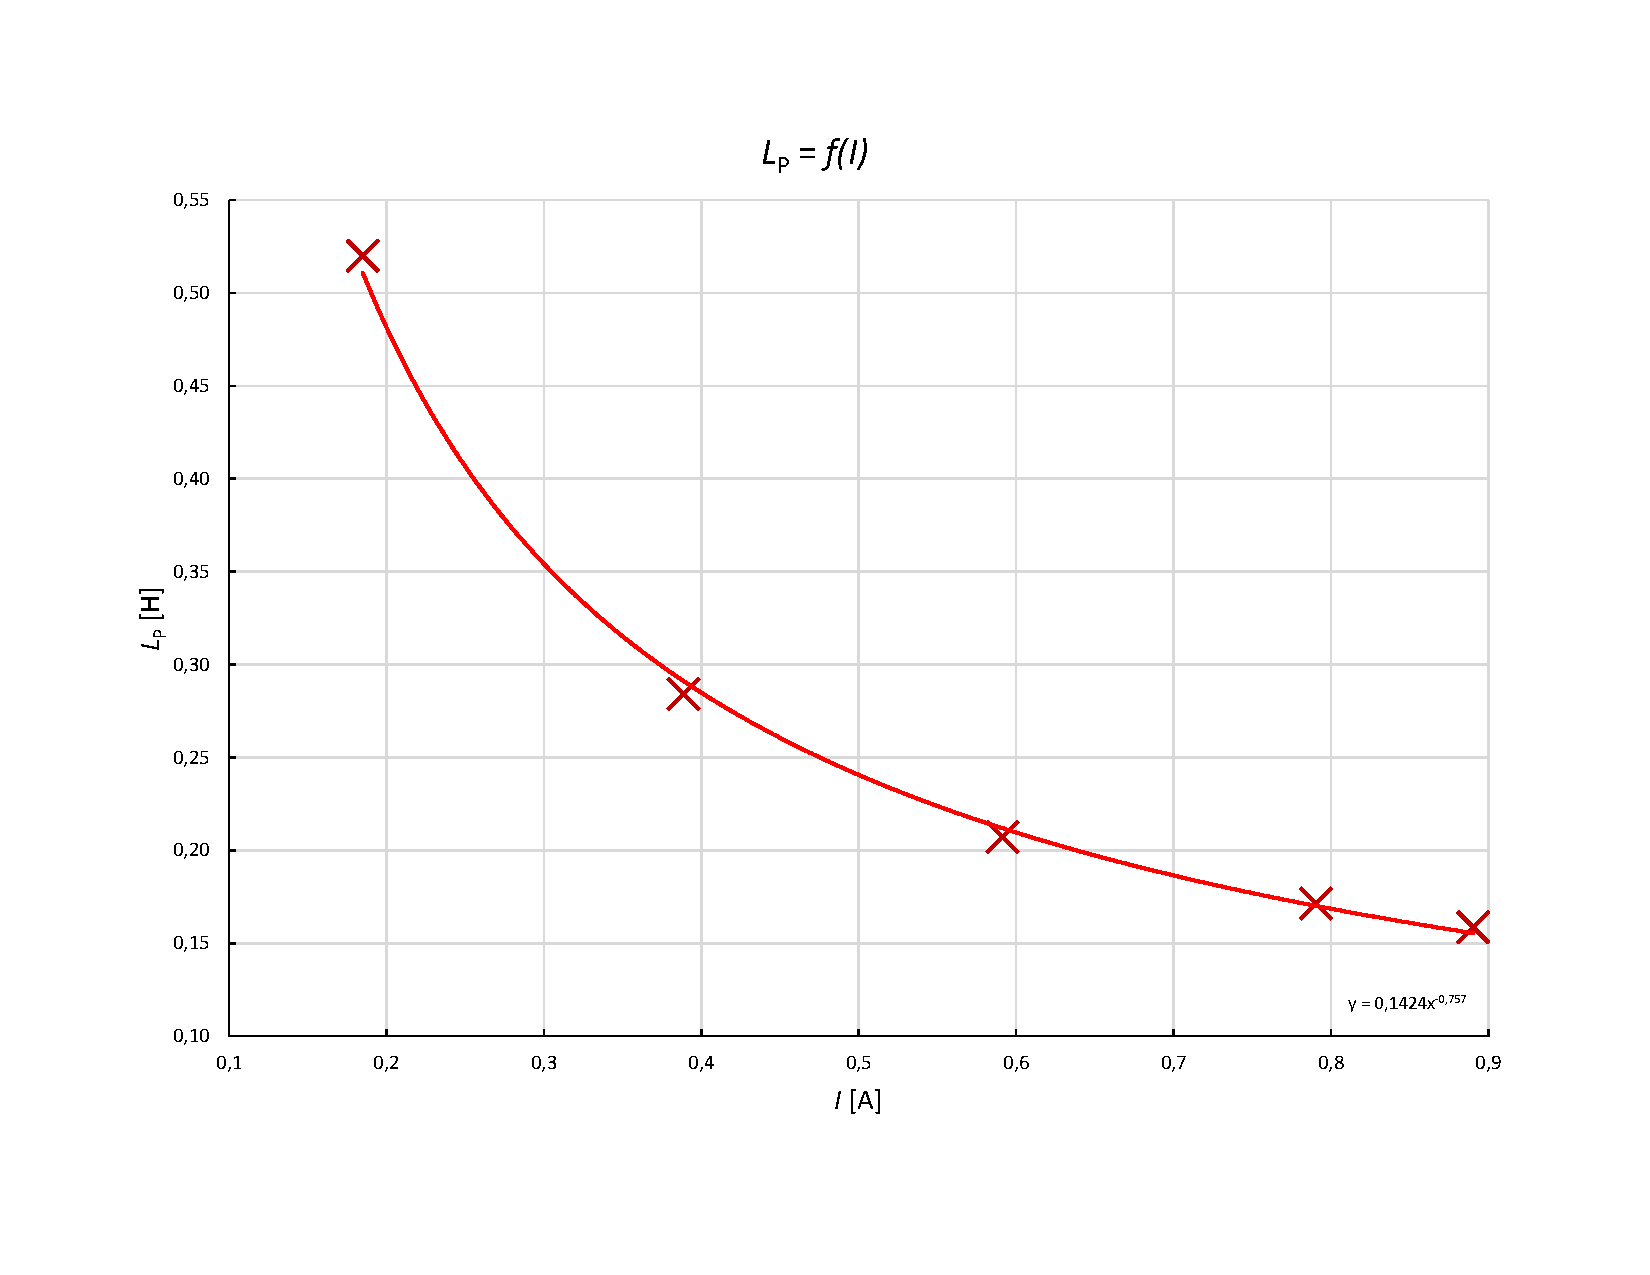
\includegraphics[width=\textwidth, trim={0 3cm 0 3cm}]{grafy/9A_graf2.pdf}
    \caption{Závislost hodnot $L_\text{P}$ paralelního náhradního schématu na sycení tlumivky}
\end{figure}

\begin{figure}[H]
    \centering
    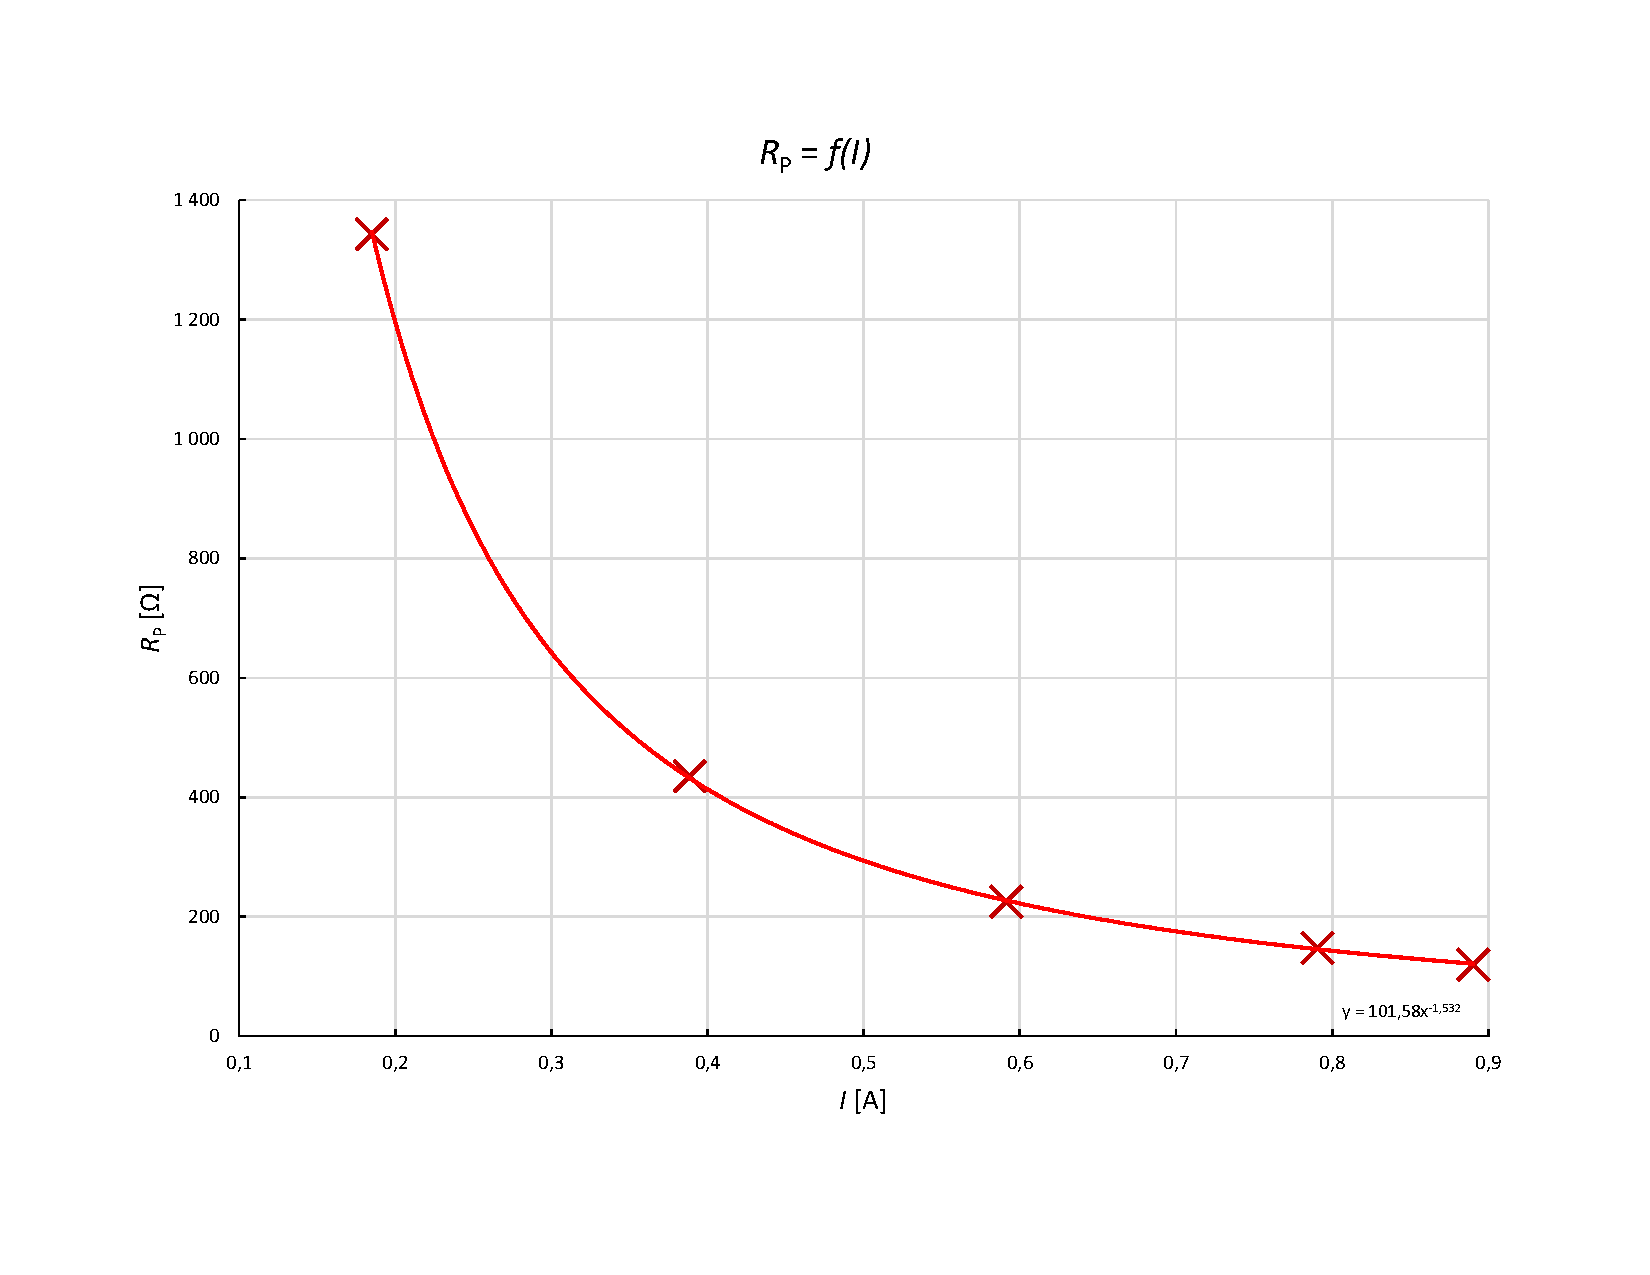
\includegraphics[width=\textwidth, trim={0 3cm 0 3cm}]{grafy/9A_graf1.pdf}
    \caption{Závislost hodnot $R_\text{P}$ paralelního náhradního schématu na sycení tlumivky}
\end{figure}

\subsection{Příklady výpočtu}

\section{Seznam použitých přístrojů}

\section{Závěr}

\end{document}